% Created by tikzDevice version 0.7.0 on 2014-11-06 12:22:47
% !TEX encoding = UTF-8 Unicode
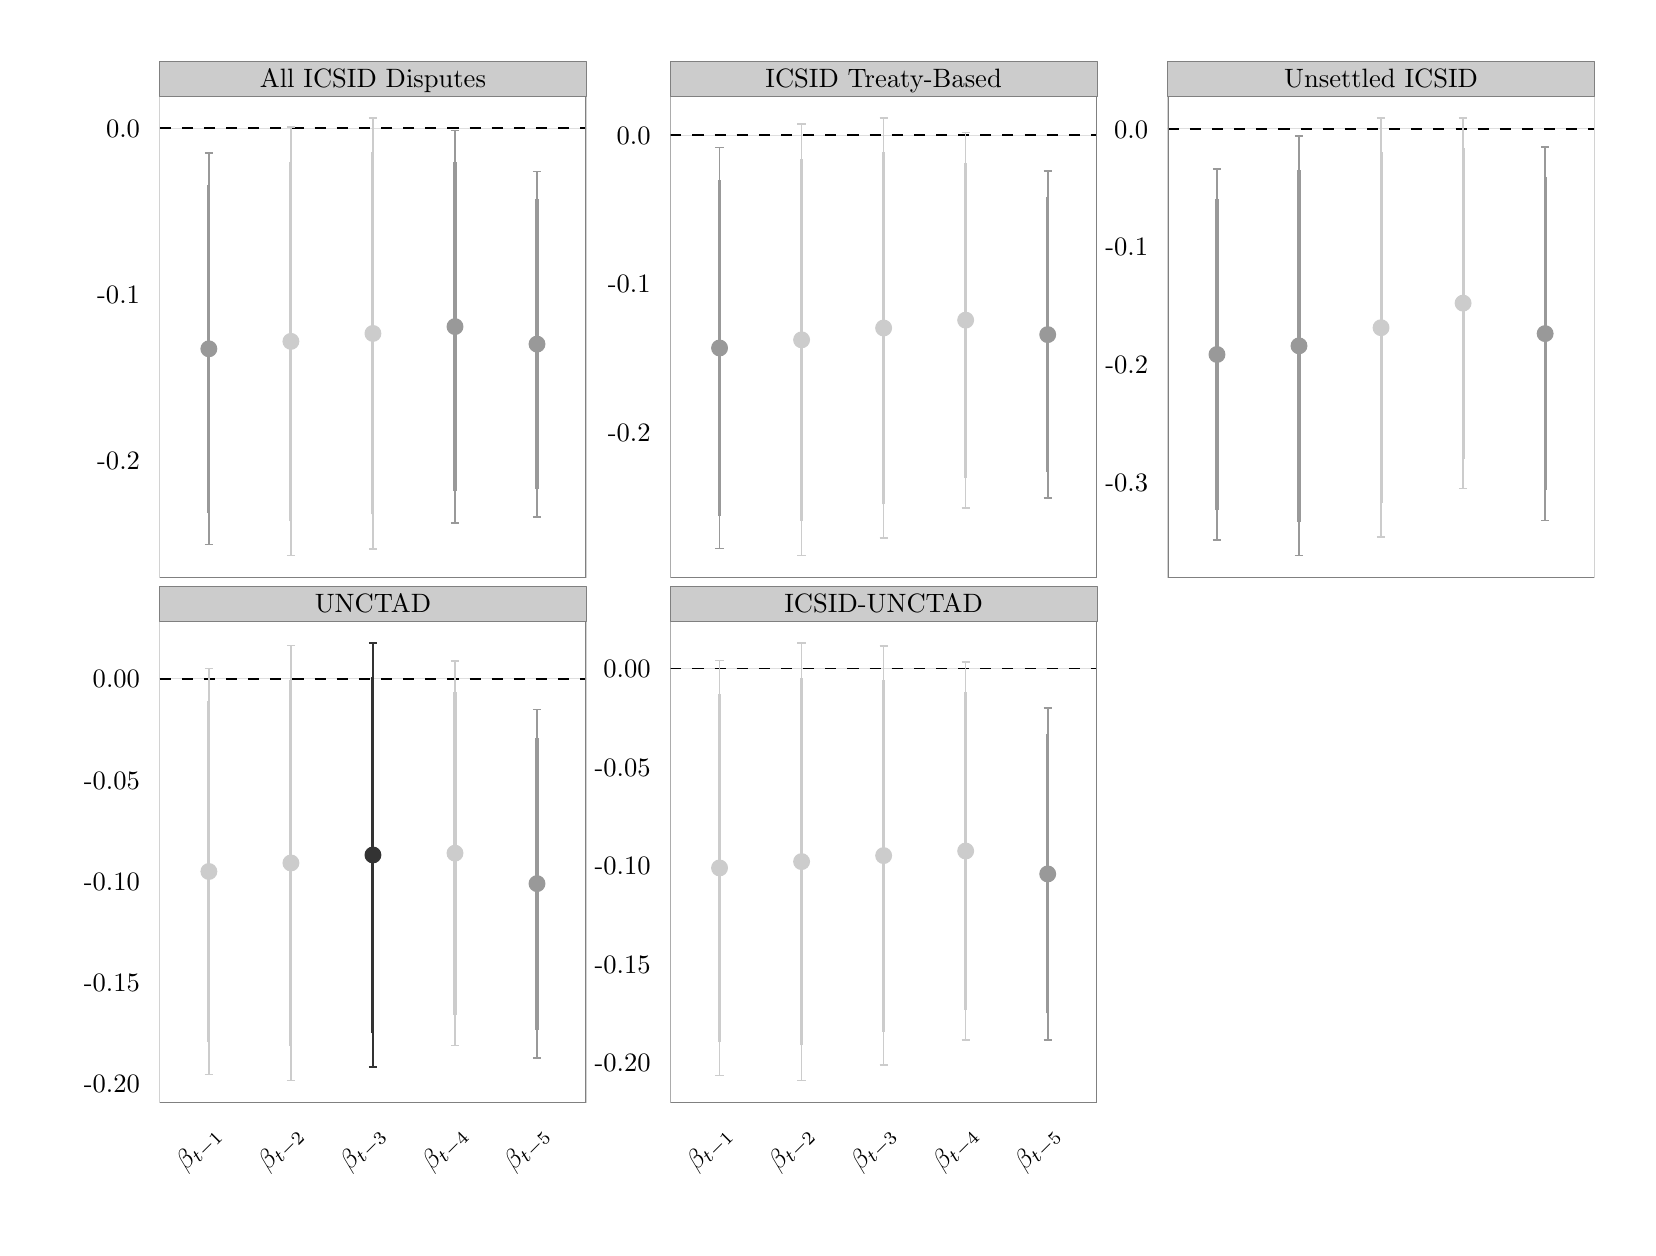
\begin{tikzpicture}[x=1pt,y=1pt]
\definecolor[named]{fillColor}{rgb}{1.00,1.00,1.00}
\path[use as bounding box,fill=fillColor,fill opacity=0.00] (0,0) rectangle (578.16,433.62);
\begin{scope}
\path[clip] (  0.00,  0.00) rectangle (578.16,433.62);
\definecolor[named]{drawColor}{rgb}{1.00,1.00,1.00}
\definecolor[named]{fillColor}{rgb}{1.00,1.00,1.00}

\path[draw=drawColor,line width= 0.6pt,line join=round,line cap=round,fill=fillColor] (  0.00,  0.00) rectangle (578.16,433.62);
\end{scope}
\begin{scope}
\path[clip] ( 47.68,234.93) rectangle (201.84,408.94);
\definecolor[named]{fillColor}{rgb}{1.00,1.00,1.00}

\path[fill=fillColor] ( 47.68,234.93) rectangle (201.84,408.94);
\definecolor[named]{drawColor}{rgb}{0.60,0.60,0.60}
\definecolor[named]{fillColor}{rgb}{0.60,0.60,0.60}

\path[draw=drawColor,draw opacity=0.30,line width= 0.3pt,line join=round,fill=fillColor,fill opacity=0.30] ( 65.47,246.83) -- ( 65.47,388.31);
\definecolor[named]{drawColor}{rgb}{0.80,0.80,0.80}
\definecolor[named]{fillColor}{rgb}{0.80,0.80,0.80}

\path[draw=drawColor,draw opacity=0.30,line width= 0.3pt,line join=round,fill=fillColor,fill opacity=0.30] ( 95.12,242.84) -- ( 95.12,397.68);

\path[draw=drawColor,draw opacity=0.30,line width= 0.3pt,line join=round,fill=fillColor,fill opacity=0.30] (124.76,245.21) -- (124.76,401.03);
\definecolor[named]{drawColor}{rgb}{0.60,0.60,0.60}
\definecolor[named]{fillColor}{rgb}{0.60,0.60,0.60}

\path[draw=drawColor,draw opacity=0.30,line width= 0.3pt,line join=round,fill=fillColor,fill opacity=0.30] (154.41,254.72) -- (154.41,396.49);

\path[draw=drawColor,draw opacity=0.30,line width= 0.3pt,line join=round,fill=fillColor,fill opacity=0.30] (184.05,256.86) -- (184.05,381.67);
\definecolor[named]{drawColor}{rgb}{0.60,0.60,0.60}
\definecolor[named]{fillColor}{rgb}{0.60,0.60,0.60}

\path[draw=drawColor,line width= 1.1pt,line join=round,fill=fillColor] ( 65.47,258.20) -- ( 65.47,376.93);
\definecolor[named]{drawColor}{rgb}{0.80,0.80,0.80}
\definecolor[named]{fillColor}{rgb}{0.80,0.80,0.80}

\path[draw=drawColor,line width= 1.1pt,line join=round,fill=fillColor] ( 95.12,255.29) -- ( 95.12,385.23);

\path[draw=drawColor,line width= 1.1pt,line join=round,fill=fillColor] (124.76,257.74) -- (124.76,388.51);
\definecolor[named]{drawColor}{rgb}{0.60,0.60,0.60}
\definecolor[named]{fillColor}{rgb}{0.60,0.60,0.60}

\path[draw=drawColor,line width= 1.1pt,line join=round,fill=fillColor] (154.41,266.11) -- (154.41,385.10);

\path[draw=drawColor,line width= 1.1pt,line join=round,fill=fillColor] (184.05,266.89) -- (184.05,371.64);
\definecolor[named]{drawColor}{rgb}{0.00,0.00,0.00}
\definecolor[named]{fillColor}{rgb}{0.00,0.00,0.00}

\path[draw=drawColor,line width= 0.6pt,dash pattern=on 4pt off 4pt ,line join=round,fill=fillColor] ( 47.68,397.32) -- (201.84,397.32);
\definecolor[named]{drawColor}{rgb}{0.60,0.60,0.60}
\definecolor[named]{fillColor}{rgb}{0.60,0.60,0.60}

\path[draw=drawColor,line width= 0.4pt,line join=round,line cap=round,fill=fillColor] ( 65.47,317.57) circle (  2.85);
\definecolor[named]{drawColor}{rgb}{0.80,0.80,0.80}
\definecolor[named]{fillColor}{rgb}{0.80,0.80,0.80}

\path[draw=drawColor,line width= 0.4pt,line join=round,line cap=round,fill=fillColor] ( 95.12,320.26) circle (  2.85);

\path[draw=drawColor,line width= 0.4pt,line join=round,line cap=round,fill=fillColor] (124.76,323.12) circle (  2.85);
\definecolor[named]{drawColor}{rgb}{0.60,0.60,0.60}
\definecolor[named]{fillColor}{rgb}{0.60,0.60,0.60}

\path[draw=drawColor,line width= 0.4pt,line join=round,line cap=round,fill=fillColor] (154.41,325.60) circle (  2.85);

\path[draw=drawColor,line width= 0.4pt,line join=round,line cap=round,fill=fillColor] (184.05,319.27) circle (  2.85);

\path[draw=drawColor,line width= 0.6pt,line join=round] ( 63.99,388.31) --
	( 66.95,388.31);

\path[draw=drawColor,line width= 0.6pt,line join=round] ( 65.47,388.31) --
	( 65.47,246.83);

\path[draw=drawColor,line width= 0.6pt,line join=round] ( 63.99,246.83) --
	( 66.95,246.83);
\definecolor[named]{drawColor}{rgb}{0.80,0.80,0.80}

\path[draw=drawColor,line width= 0.6pt,line join=round] ( 93.63,397.68) --
	( 96.60,397.68);

\path[draw=drawColor,line width= 0.6pt,line join=round] ( 95.12,397.68) --
	( 95.12,242.84);

\path[draw=drawColor,line width= 0.6pt,line join=round] ( 93.63,242.84) --
	( 96.60,242.84);

\path[draw=drawColor,line width= 0.6pt,line join=round] (123.28,401.03) --
	(126.24,401.03);

\path[draw=drawColor,line width= 0.6pt,line join=round] (124.76,401.03) --
	(124.76,245.21);

\path[draw=drawColor,line width= 0.6pt,line join=round] (123.28,245.21) --
	(126.24,245.21);
\definecolor[named]{drawColor}{rgb}{0.60,0.60,0.60}

\path[draw=drawColor,line width= 0.6pt,line join=round] (152.92,396.49) --
	(155.89,396.49);

\path[draw=drawColor,line width= 0.6pt,line join=round] (154.41,396.49) --
	(154.41,254.72);

\path[draw=drawColor,line width= 0.6pt,line join=round] (152.92,254.72) --
	(155.89,254.72);

\path[draw=drawColor,line width= 0.6pt,line join=round] (182.57,381.67) --
	(185.53,381.67);

\path[draw=drawColor,line width= 0.6pt,line join=round] (184.05,381.67) --
	(184.05,256.86);

\path[draw=drawColor,line width= 0.6pt,line join=round] (182.57,256.86) --
	(185.53,256.86);
\definecolor[named]{drawColor}{rgb}{0.50,0.50,0.50}

\path[draw=drawColor,line width= 0.6pt,line join=round,line cap=round] ( 47.68,234.93) rectangle (201.84,408.94);
\end{scope}
\begin{scope}
\path[clip] (232.22,234.93) rectangle (386.38,408.94);
\definecolor[named]{fillColor}{rgb}{1.00,1.00,1.00}

\path[fill=fillColor] (232.22,234.93) rectangle (386.38,408.94);
\definecolor[named]{drawColor}{rgb}{0.60,0.60,0.60}
\definecolor[named]{fillColor}{rgb}{0.60,0.60,0.60}

\path[draw=drawColor,draw opacity=0.30,line width= 0.3pt,line join=round,fill=fillColor,fill opacity=0.30] (250.01,245.44) -- (250.01,390.30);
\definecolor[named]{drawColor}{rgb}{0.80,0.80,0.80}
\definecolor[named]{fillColor}{rgb}{0.80,0.80,0.80}

\path[draw=drawColor,draw opacity=0.30,line width= 0.3pt,line join=round,fill=fillColor,fill opacity=0.30] (279.65,242.84) -- (279.65,398.79);

\path[draw=drawColor,draw opacity=0.30,line width= 0.3pt,line join=round,fill=fillColor,fill opacity=0.30] (309.30,249.14) -- (309.30,401.03);

\path[draw=drawColor,draw opacity=0.30,line width= 0.3pt,line join=round,fill=fillColor,fill opacity=0.30] (338.94,260.12) -- (338.94,395.73);
\definecolor[named]{drawColor}{rgb}{0.60,0.60,0.60}
\definecolor[named]{fillColor}{rgb}{0.60,0.60,0.60}

\path[draw=drawColor,draw opacity=0.30,line width= 0.3pt,line join=round,fill=fillColor,fill opacity=0.30] (368.59,263.56) -- (368.59,381.85);
\definecolor[named]{drawColor}{rgb}{0.60,0.60,0.60}
\definecolor[named]{fillColor}{rgb}{0.60,0.60,0.60}

\path[draw=drawColor,line width= 1.1pt,line join=round,fill=fillColor] (250.01,257.08) -- (250.01,378.65);
\definecolor[named]{drawColor}{rgb}{0.80,0.80,0.80}
\definecolor[named]{fillColor}{rgb}{0.80,0.80,0.80}

\path[draw=drawColor,line width= 1.1pt,line join=round,fill=fillColor] (279.65,255.38) -- (279.65,386.25);

\path[draw=drawColor,line width= 1.1pt,line join=round,fill=fillColor] (309.30,261.35) -- (309.30,388.82);

\path[draw=drawColor,line width= 1.1pt,line join=round,fill=fillColor] (338.94,271.02) -- (338.94,384.83);
\definecolor[named]{drawColor}{rgb}{0.60,0.60,0.60}
\definecolor[named]{fillColor}{rgb}{0.60,0.60,0.60}

\path[draw=drawColor,line width= 1.1pt,line join=round,fill=fillColor] (368.59,273.07) -- (368.59,372.34);
\definecolor[named]{drawColor}{rgb}{0.00,0.00,0.00}
\definecolor[named]{fillColor}{rgb}{0.00,0.00,0.00}

\path[draw=drawColor,line width= 0.6pt,dash pattern=on 4pt off 4pt ,line join=round,fill=fillColor] (232.22,394.80) -- (386.38,394.80);
\definecolor[named]{drawColor}{rgb}{0.60,0.60,0.60}
\definecolor[named]{fillColor}{rgb}{0.60,0.60,0.60}

\path[draw=drawColor,line width= 0.4pt,line join=round,line cap=round,fill=fillColor] (250.01,317.87) circle (  2.85);
\definecolor[named]{drawColor}{rgb}{0.80,0.80,0.80}
\definecolor[named]{fillColor}{rgb}{0.80,0.80,0.80}

\path[draw=drawColor,line width= 0.4pt,line join=round,line cap=round,fill=fillColor] (279.65,320.81) circle (  2.85);

\path[draw=drawColor,line width= 0.4pt,line join=round,line cap=round,fill=fillColor] (309.30,325.09) circle (  2.85);

\path[draw=drawColor,line width= 0.4pt,line join=round,line cap=round,fill=fillColor] (338.94,327.93) circle (  2.85);
\definecolor[named]{drawColor}{rgb}{0.60,0.60,0.60}
\definecolor[named]{fillColor}{rgb}{0.60,0.60,0.60}

\path[draw=drawColor,line width= 0.4pt,line join=round,line cap=round,fill=fillColor] (368.59,322.70) circle (  2.85);

\path[draw=drawColor,line width= 0.6pt,line join=round] (248.53,390.30) --
	(251.49,390.30);

\path[draw=drawColor,line width= 0.6pt,line join=round] (250.01,390.30) --
	(250.01,245.44);

\path[draw=drawColor,line width= 0.6pt,line join=round] (248.53,245.44) --
	(251.49,245.44);
\definecolor[named]{drawColor}{rgb}{0.80,0.80,0.80}

\path[draw=drawColor,line width= 0.6pt,line join=round] (278.17,398.79) --
	(281.14,398.79);

\path[draw=drawColor,line width= 0.6pt,line join=round] (279.65,398.79) --
	(279.65,242.84);

\path[draw=drawColor,line width= 0.6pt,line join=round] (278.17,242.84) --
	(281.14,242.84);

\path[draw=drawColor,line width= 0.6pt,line join=round] (307.82,401.03) --
	(310.78,401.03);

\path[draw=drawColor,line width= 0.6pt,line join=round] (309.30,401.03) --
	(309.30,249.14);

\path[draw=drawColor,line width= 0.6pt,line join=round] (307.82,249.14) --
	(310.78,249.14);

\path[draw=drawColor,line width= 0.6pt,line join=round] (337.46,395.73) --
	(340.43,395.73);

\path[draw=drawColor,line width= 0.6pt,line join=round] (338.94,395.73) --
	(338.94,260.12);

\path[draw=drawColor,line width= 0.6pt,line join=round] (337.46,260.12) --
	(340.43,260.12);
\definecolor[named]{drawColor}{rgb}{0.60,0.60,0.60}

\path[draw=drawColor,line width= 0.6pt,line join=round] (367.11,381.85) --
	(370.07,381.85);

\path[draw=drawColor,line width= 0.6pt,line join=round] (368.59,381.85) --
	(368.59,263.56);

\path[draw=drawColor,line width= 0.6pt,line join=round] (367.11,263.56) --
	(370.07,263.56);
\definecolor[named]{drawColor}{rgb}{0.50,0.50,0.50}

\path[draw=drawColor,line width= 0.6pt,line join=round,line cap=round] (232.22,234.93) rectangle (386.38,408.94);
\end{scope}
\begin{scope}
\path[clip] (411.96,234.93) rectangle (566.12,408.94);
\definecolor[named]{fillColor}{rgb}{1.00,1.00,1.00}

\path[fill=fillColor] (411.96,234.93) rectangle (566.12,408.94);
\definecolor[named]{drawColor}{rgb}{0.60,0.60,0.60}
\definecolor[named]{fillColor}{rgb}{0.60,0.60,0.60}

\path[draw=drawColor,draw opacity=0.30,line width= 0.3pt,line join=round,fill=fillColor,fill opacity=0.30] (429.75,248.53) -- (429.75,382.50);

\path[draw=drawColor,draw opacity=0.30,line width= 0.3pt,line join=round,fill=fillColor,fill opacity=0.30] (459.39,242.84) -- (459.39,394.45);
\definecolor[named]{drawColor}{rgb}{0.80,0.80,0.80}
\definecolor[named]{fillColor}{rgb}{0.80,0.80,0.80}

\path[draw=drawColor,draw opacity=0.30,line width= 0.3pt,line join=round,fill=fillColor,fill opacity=0.30] (489.04,249.51) -- (489.04,400.89);

\path[draw=drawColor,draw opacity=0.30,line width= 0.3pt,line join=round,fill=fillColor,fill opacity=0.30] (518.68,267.14) -- (518.68,401.03);
\definecolor[named]{drawColor}{rgb}{0.60,0.60,0.60}
\definecolor[named]{fillColor}{rgb}{0.60,0.60,0.60}

\path[draw=drawColor,draw opacity=0.30,line width= 0.3pt,line join=round,fill=fillColor,fill opacity=0.30] (548.33,255.55) -- (548.33,390.59);
\definecolor[named]{drawColor}{rgb}{0.60,0.60,0.60}
\definecolor[named]{fillColor}{rgb}{0.60,0.60,0.60}

\path[draw=drawColor,line width= 1.1pt,line join=round,fill=fillColor] (429.75,259.30) -- (429.75,371.74);

\path[draw=drawColor,line width= 1.1pt,line join=round,fill=fillColor] (459.39,255.03) -- (459.39,382.27);
\definecolor[named]{drawColor}{rgb}{0.80,0.80,0.80}
\definecolor[named]{fillColor}{rgb}{0.80,0.80,0.80}

\path[draw=drawColor,line width= 1.1pt,line join=round,fill=fillColor] (489.04,261.68) -- (489.04,388.72);

\path[draw=drawColor,line width= 1.1pt,line join=round,fill=fillColor] (518.68,277.90) -- (518.68,390.27);
\definecolor[named]{drawColor}{rgb}{0.60,0.60,0.60}
\definecolor[named]{fillColor}{rgb}{0.60,0.60,0.60}

\path[draw=drawColor,line width= 1.1pt,line join=round,fill=fillColor] (548.33,266.40) -- (548.33,379.73);
\definecolor[named]{drawColor}{rgb}{0.00,0.00,0.00}
\definecolor[named]{fillColor}{rgb}{0.00,0.00,0.00}

\path[draw=drawColor,line width= 0.6pt,dash pattern=on 4pt off 4pt ,line join=round,fill=fillColor] (411.96,397.03) -- (566.12,397.03);
\definecolor[named]{drawColor}{rgb}{0.60,0.60,0.60}
\definecolor[named]{fillColor}{rgb}{0.60,0.60,0.60}

\path[draw=drawColor,line width= 0.4pt,line join=round,line cap=round,fill=fillColor] (429.75,315.52) circle (  2.85);

\path[draw=drawColor,line width= 0.4pt,line join=round,line cap=round,fill=fillColor] (459.39,318.65) circle (  2.85);
\definecolor[named]{drawColor}{rgb}{0.80,0.80,0.80}
\definecolor[named]{fillColor}{rgb}{0.80,0.80,0.80}

\path[draw=drawColor,line width= 0.4pt,line join=round,line cap=round,fill=fillColor] (489.04,325.20) circle (  2.85);

\path[draw=drawColor,line width= 0.4pt,line join=round,line cap=round,fill=fillColor] (518.68,334.08) circle (  2.85);
\definecolor[named]{drawColor}{rgb}{0.60,0.60,0.60}
\definecolor[named]{fillColor}{rgb}{0.60,0.60,0.60}

\path[draw=drawColor,line width= 0.4pt,line join=round,line cap=round,fill=fillColor] (548.33,323.07) circle (  2.85);

\path[draw=drawColor,line width= 0.6pt,line join=round] (428.27,382.50) --
	(431.23,382.50);

\path[draw=drawColor,line width= 0.6pt,line join=round] (429.75,382.50) --
	(429.75,248.53);

\path[draw=drawColor,line width= 0.6pt,line join=round] (428.27,248.53) --
	(431.23,248.53);

\path[draw=drawColor,line width= 0.6pt,line join=round] (457.91,394.45) --
	(460.88,394.45);

\path[draw=drawColor,line width= 0.6pt,line join=round] (459.39,394.45) --
	(459.39,242.84);

\path[draw=drawColor,line width= 0.6pt,line join=round] (457.91,242.84) --
	(460.88,242.84);
\definecolor[named]{drawColor}{rgb}{0.80,0.80,0.80}

\path[draw=drawColor,line width= 0.6pt,line join=round] (487.56,400.89) --
	(490.52,400.89);

\path[draw=drawColor,line width= 0.6pt,line join=round] (489.04,400.89) --
	(489.04,249.51);

\path[draw=drawColor,line width= 0.6pt,line join=round] (487.56,249.51) --
	(490.52,249.51);

\path[draw=drawColor,line width= 0.6pt,line join=round] (517.20,401.03) --
	(520.17,401.03);

\path[draw=drawColor,line width= 0.6pt,line join=round] (518.68,401.03) --
	(518.68,267.14);

\path[draw=drawColor,line width= 0.6pt,line join=round] (517.20,267.14) --
	(520.17,267.14);
\definecolor[named]{drawColor}{rgb}{0.60,0.60,0.60}

\path[draw=drawColor,line width= 0.6pt,line join=round] (546.85,390.59) --
	(549.81,390.59);

\path[draw=drawColor,line width= 0.6pt,line join=round] (548.33,390.59) --
	(548.33,255.55);

\path[draw=drawColor,line width= 0.6pt,line join=round] (546.85,255.55) --
	(549.81,255.55);
\definecolor[named]{drawColor}{rgb}{0.50,0.50,0.50}

\path[draw=drawColor,line width= 0.6pt,line join=round,line cap=round] (411.96,234.93) rectangle (566.12,408.94);
\end{scope}
\begin{scope}
\path[clip] ( 47.68, 45.28) rectangle (201.84,219.29);
\definecolor[named]{fillColor}{rgb}{1.00,1.00,1.00}

\path[fill=fillColor] ( 47.68, 45.28) rectangle (201.84,219.29);
\definecolor[named]{drawColor}{rgb}{0.80,0.80,0.80}
\definecolor[named]{fillColor}{rgb}{0.80,0.80,0.80}

\path[draw=drawColor,draw opacity=0.30,line width= 0.3pt,line join=round,fill=fillColor,fill opacity=0.30] ( 65.47, 55.29) -- ( 65.47,202.10);

\path[draw=drawColor,draw opacity=0.30,line width= 0.3pt,line join=round,fill=fillColor,fill opacity=0.30] ( 95.12, 53.19) -- ( 95.12,210.38);
\definecolor[named]{drawColor}{rgb}{0.20,0.20,0.20}
\definecolor[named]{fillColor}{rgb}{0.20,0.20,0.20}

\path[draw=drawColor,draw opacity=0.30,line width= 0.3pt,line join=round,fill=fillColor,fill opacity=0.30] (124.76, 57.96) -- (124.76,211.38);
\definecolor[named]{drawColor}{rgb}{0.80,0.80,0.80}
\definecolor[named]{fillColor}{rgb}{0.80,0.80,0.80}

\path[draw=drawColor,draw opacity=0.30,line width= 0.3pt,line join=round,fill=fillColor,fill opacity=0.30] (154.41, 65.79) -- (154.41,204.84);
\definecolor[named]{drawColor}{rgb}{0.60,0.60,0.60}
\definecolor[named]{fillColor}{rgb}{0.60,0.60,0.60}

\path[draw=drawColor,draw opacity=0.30,line width= 0.3pt,line join=round,fill=fillColor,fill opacity=0.30] (184.05, 61.42) -- (184.05,187.23);
\definecolor[named]{drawColor}{rgb}{0.80,0.80,0.80}
\definecolor[named]{fillColor}{rgb}{0.80,0.80,0.80}

\path[draw=drawColor,line width= 1.1pt,line join=round,fill=fillColor] ( 65.47, 67.09) -- ( 65.47,190.30);

\path[draw=drawColor,line width= 1.1pt,line join=round,fill=fillColor] ( 95.12, 65.82) -- ( 95.12,197.74);
\definecolor[named]{drawColor}{rgb}{0.20,0.20,0.20}
\definecolor[named]{fillColor}{rgb}{0.20,0.20,0.20}

\path[draw=drawColor,line width= 1.1pt,line join=round,fill=fillColor] (124.76, 70.30) -- (124.76,199.04);
\definecolor[named]{drawColor}{rgb}{0.80,0.80,0.80}
\definecolor[named]{fillColor}{rgb}{0.80,0.80,0.80}

\path[draw=drawColor,line width= 1.1pt,line join=round,fill=fillColor] (154.41, 76.97) -- (154.41,193.67);
\definecolor[named]{drawColor}{rgb}{0.60,0.60,0.60}
\definecolor[named]{fillColor}{rgb}{0.60,0.60,0.60}

\path[draw=drawColor,line width= 1.1pt,line join=round,fill=fillColor] (184.05, 71.53) -- (184.05,177.11);
\definecolor[named]{drawColor}{rgb}{0.00,0.00,0.00}
\definecolor[named]{fillColor}{rgb}{0.00,0.00,0.00}

\path[draw=drawColor,line width= 0.6pt,dash pattern=on 4pt off 4pt ,line join=round,fill=fillColor] ( 47.68,198.32) -- (201.84,198.32);
\definecolor[named]{drawColor}{rgb}{0.80,0.80,0.80}
\definecolor[named]{fillColor}{rgb}{0.80,0.80,0.80}

\path[draw=drawColor,line width= 0.4pt,line join=round,line cap=round,fill=fillColor] ( 65.47,128.70) circle (  2.85);

\path[draw=drawColor,line width= 0.4pt,line join=round,line cap=round,fill=fillColor] ( 95.12,131.78) circle (  2.85);
\definecolor[named]{drawColor}{rgb}{0.20,0.20,0.20}
\definecolor[named]{fillColor}{rgb}{0.20,0.20,0.20}

\path[draw=drawColor,line width= 0.4pt,line join=round,line cap=round,fill=fillColor] (124.76,134.67) circle (  2.85);
\definecolor[named]{drawColor}{rgb}{0.80,0.80,0.80}
\definecolor[named]{fillColor}{rgb}{0.80,0.80,0.80}

\path[draw=drawColor,line width= 0.4pt,line join=round,line cap=round,fill=fillColor] (154.41,135.32) circle (  2.85);
\definecolor[named]{drawColor}{rgb}{0.60,0.60,0.60}
\definecolor[named]{fillColor}{rgb}{0.60,0.60,0.60}

\path[draw=drawColor,line width= 0.4pt,line join=round,line cap=round,fill=fillColor] (184.05,124.32) circle (  2.85);
\definecolor[named]{drawColor}{rgb}{0.80,0.80,0.80}

\path[draw=drawColor,line width= 0.6pt,line join=round] ( 63.99,202.10) --
	( 66.95,202.10);

\path[draw=drawColor,line width= 0.6pt,line join=round] ( 65.47,202.10) --
	( 65.47, 55.29);

\path[draw=drawColor,line width= 0.6pt,line join=round] ( 63.99, 55.29) --
	( 66.95, 55.29);

\path[draw=drawColor,line width= 0.6pt,line join=round] ( 93.63,210.38) --
	( 96.60,210.38);

\path[draw=drawColor,line width= 0.6pt,line join=round] ( 95.12,210.38) --
	( 95.12, 53.19);

\path[draw=drawColor,line width= 0.6pt,line join=round] ( 93.63, 53.19) --
	( 96.60, 53.19);
\definecolor[named]{drawColor}{rgb}{0.20,0.20,0.20}

\path[draw=drawColor,line width= 0.6pt,line join=round] (123.28,211.38) --
	(126.24,211.38);

\path[draw=drawColor,line width= 0.6pt,line join=round] (124.76,211.38) --
	(124.76, 57.96);

\path[draw=drawColor,line width= 0.6pt,line join=round] (123.28, 57.96) --
	(126.24, 57.96);
\definecolor[named]{drawColor}{rgb}{0.80,0.80,0.80}

\path[draw=drawColor,line width= 0.6pt,line join=round] (152.92,204.84) --
	(155.89,204.84);

\path[draw=drawColor,line width= 0.6pt,line join=round] (154.41,204.84) --
	(154.41, 65.79);

\path[draw=drawColor,line width= 0.6pt,line join=round] (152.92, 65.79) --
	(155.89, 65.79);
\definecolor[named]{drawColor}{rgb}{0.60,0.60,0.60}

\path[draw=drawColor,line width= 0.6pt,line join=round] (182.57,187.23) --
	(185.53,187.23);

\path[draw=drawColor,line width= 0.6pt,line join=round] (184.05,187.23) --
	(184.05, 61.42);

\path[draw=drawColor,line width= 0.6pt,line join=round] (182.57, 61.42) --
	(185.53, 61.42);
\definecolor[named]{drawColor}{rgb}{0.50,0.50,0.50}

\path[draw=drawColor,line width= 0.6pt,line join=round,line cap=round] ( 47.68, 45.28) rectangle (201.84,219.29);
\end{scope}
\begin{scope}
\path[clip] (232.22, 45.28) rectangle (386.38,219.29);
\definecolor[named]{fillColor}{rgb}{1.00,1.00,1.00}

\path[fill=fillColor] (232.22, 45.28) rectangle (386.38,219.29);
\definecolor[named]{drawColor}{rgb}{0.80,0.80,0.80}
\definecolor[named]{fillColor}{rgb}{0.80,0.80,0.80}

\path[draw=drawColor,draw opacity=0.30,line width= 0.3pt,line join=round,fill=fillColor,fill opacity=0.30] (250.01, 55.04) -- (250.01,204.94);

\path[draw=drawColor,draw opacity=0.30,line width= 0.3pt,line join=round,fill=fillColor,fill opacity=0.30] (279.65, 53.19) -- (279.65,211.38);

\path[draw=drawColor,draw opacity=0.30,line width= 0.3pt,line join=round,fill=fillColor,fill opacity=0.30] (309.30, 58.67) -- (309.30,210.23);

\path[draw=drawColor,draw opacity=0.30,line width= 0.3pt,line join=round,fill=fillColor,fill opacity=0.30] (338.94, 67.70) -- (338.94,204.50);
\definecolor[named]{drawColor}{rgb}{0.60,0.60,0.60}
\definecolor[named]{fillColor}{rgb}{0.60,0.60,0.60}

\path[draw=drawColor,draw opacity=0.30,line width= 0.3pt,line join=round,fill=fillColor,fill opacity=0.30] (368.59, 67.74) -- (368.59,187.89);
\definecolor[named]{drawColor}{rgb}{0.80,0.80,0.80}
\definecolor[named]{fillColor}{rgb}{0.80,0.80,0.80}

\path[draw=drawColor,line width= 1.1pt,line join=round,fill=fillColor] (250.01, 67.09) -- (250.01,192.89);

\path[draw=drawColor,line width= 1.1pt,line join=round,fill=fillColor] (279.65, 65.90) -- (279.65,198.66);

\path[draw=drawColor,line width= 1.1pt,line join=round,fill=fillColor] (309.30, 70.86) -- (309.30,198.05);

\path[draw=drawColor,line width= 1.1pt,line join=round,fill=fillColor] (338.94, 78.70) -- (338.94,193.51);
\definecolor[named]{drawColor}{rgb}{0.60,0.60,0.60}
\definecolor[named]{fillColor}{rgb}{0.60,0.60,0.60}

\path[draw=drawColor,line width= 1.1pt,line join=round,fill=fillColor] (368.59, 77.40) -- (368.59,178.23);
\definecolor[named]{drawColor}{rgb}{0.00,0.00,0.00}
\definecolor[named]{fillColor}{rgb}{0.00,0.00,0.00}

\path[draw=drawColor,line width= 0.6pt,dash pattern=on 4pt off 4pt ,line join=round,fill=fillColor] (232.22,202.07) -- (386.38,202.07);
\definecolor[named]{drawColor}{rgb}{0.80,0.80,0.80}
\definecolor[named]{fillColor}{rgb}{0.80,0.80,0.80}

\path[draw=drawColor,line width= 0.4pt,line join=round,line cap=round,fill=fillColor] (250.01,129.99) circle (  2.85);

\path[draw=drawColor,line width= 0.4pt,line join=round,line cap=round,fill=fillColor] (279.65,132.28) circle (  2.85);

\path[draw=drawColor,line width= 0.4pt,line join=round,line cap=round,fill=fillColor] (309.30,134.45) circle (  2.85);

\path[draw=drawColor,line width= 0.4pt,line join=round,line cap=round,fill=fillColor] (338.94,136.10) circle (  2.85);
\definecolor[named]{drawColor}{rgb}{0.60,0.60,0.60}
\definecolor[named]{fillColor}{rgb}{0.60,0.60,0.60}

\path[draw=drawColor,line width= 0.4pt,line join=round,line cap=round,fill=fillColor] (368.59,127.82) circle (  2.85);
\definecolor[named]{drawColor}{rgb}{0.80,0.80,0.80}

\path[draw=drawColor,line width= 0.6pt,line join=round] (248.53,204.94) --
	(251.49,204.94);

\path[draw=drawColor,line width= 0.6pt,line join=round] (250.01,204.94) --
	(250.01, 55.04);

\path[draw=drawColor,line width= 0.6pt,line join=round] (248.53, 55.04) --
	(251.49, 55.04);

\path[draw=drawColor,line width= 0.6pt,line join=round] (278.17,211.38) --
	(281.14,211.38);

\path[draw=drawColor,line width= 0.6pt,line join=round] (279.65,211.38) --
	(279.65, 53.19);

\path[draw=drawColor,line width= 0.6pt,line join=round] (278.17, 53.19) --
	(281.14, 53.19);

\path[draw=drawColor,line width= 0.6pt,line join=round] (307.82,210.23) --
	(310.78,210.23);

\path[draw=drawColor,line width= 0.6pt,line join=round] (309.30,210.23) --
	(309.30, 58.67);

\path[draw=drawColor,line width= 0.6pt,line join=round] (307.82, 58.67) --
	(310.78, 58.67);

\path[draw=drawColor,line width= 0.6pt,line join=round] (337.46,204.50) --
	(340.43,204.50);

\path[draw=drawColor,line width= 0.6pt,line join=round] (338.94,204.50) --
	(338.94, 67.70);

\path[draw=drawColor,line width= 0.6pt,line join=round] (337.46, 67.70) --
	(340.43, 67.70);
\definecolor[named]{drawColor}{rgb}{0.60,0.60,0.60}

\path[draw=drawColor,line width= 0.6pt,line join=round] (367.11,187.89) --
	(370.07,187.89);

\path[draw=drawColor,line width= 0.6pt,line join=round] (368.59,187.89) --
	(368.59, 67.74);

\path[draw=drawColor,line width= 0.6pt,line join=round] (367.11, 67.74) --
	(370.07, 67.74);
\definecolor[named]{drawColor}{rgb}{0.50,0.50,0.50}

\path[draw=drawColor,line width= 0.6pt,line join=round,line cap=round] (232.22, 45.28) rectangle (386.38,219.29);
\end{scope}
\begin{scope}
\path[clip] (  0.00,  0.00) rectangle (578.16,433.62);
\definecolor[named]{drawColor}{rgb}{0.50,0.50,0.50}
\definecolor[named]{fillColor}{rgb}{0.80,0.80,0.80}

\path[draw=drawColor,line width= 0.2pt,line join=round,line cap=round,fill=fillColor] ( 47.68,408.94) rectangle (201.84,421.57);
\definecolor[named]{drawColor}{rgb}{0.00,0.00,0.00}

\node[text=drawColor,anchor=base,inner sep=0pt, outer sep=0pt, scale=  0.96] at (124.76,411.95) {All ICSID Disputes};
\end{scope}
\begin{scope}
\path[clip] (  0.00,  0.00) rectangle (578.16,433.62);
\definecolor[named]{drawColor}{rgb}{0.50,0.50,0.50}
\definecolor[named]{fillColor}{rgb}{0.80,0.80,0.80}

\path[draw=drawColor,line width= 0.2pt,line join=round,line cap=round,fill=fillColor] (232.22,408.94) rectangle (386.38,421.57);
\definecolor[named]{drawColor}{rgb}{0.00,0.00,0.00}

\node[text=drawColor,anchor=base,inner sep=0pt, outer sep=0pt, scale=  0.96] at (309.30,411.95) {ICSID Treaty-Based};
\end{scope}
\begin{scope}
\path[clip] (  0.00,  0.00) rectangle (578.16,433.62);
\definecolor[named]{drawColor}{rgb}{0.50,0.50,0.50}
\definecolor[named]{fillColor}{rgb}{0.80,0.80,0.80}

\path[draw=drawColor,line width= 0.2pt,line join=round,line cap=round,fill=fillColor] (411.96,408.94) rectangle (566.12,421.57);
\definecolor[named]{drawColor}{rgb}{0.00,0.00,0.00}

\node[text=drawColor,anchor=base,inner sep=0pt, outer sep=0pt, scale=  0.96] at (489.04,411.95) {Unsettled ICSID};
\end{scope}
\begin{scope}
\path[clip] (  0.00,  0.00) rectangle (578.16,433.62);
\definecolor[named]{drawColor}{rgb}{0.50,0.50,0.50}
\definecolor[named]{fillColor}{rgb}{0.80,0.80,0.80}

\path[draw=drawColor,line width= 0.2pt,line join=round,line cap=round,fill=fillColor] ( 47.68,219.29) rectangle (201.84,231.92);
\definecolor[named]{drawColor}{rgb}{0.00,0.00,0.00}

\node[text=drawColor,anchor=base,inner sep=0pt, outer sep=0pt, scale=  0.96] at (124.76,222.30) {UNCTAD};
\end{scope}
\begin{scope}
\path[clip] (  0.00,  0.00) rectangle (578.16,433.62);
\definecolor[named]{drawColor}{rgb}{0.50,0.50,0.50}
\definecolor[named]{fillColor}{rgb}{0.80,0.80,0.80}

\path[draw=drawColor,line width= 0.2pt,line join=round,line cap=round,fill=fillColor] (232.22,219.29) rectangle (386.38,231.92);
\definecolor[named]{drawColor}{rgb}{0.00,0.00,0.00}

\node[text=drawColor,anchor=base,inner sep=0pt, outer sep=0pt, scale=  0.96] at (309.30,222.30) {ICSID-UNCTAD};
\end{scope}
\begin{scope}
\path[clip] (  0.00,  0.00) rectangle (578.16,433.62);
\definecolor[named]{drawColor}{rgb}{0.00,0.00,0.00}

\node[text=drawColor,anchor=base east,inner sep=0pt, outer sep=0pt, scale=  0.96] at ( 40.57,274.09) {-0.2};

\node[text=drawColor,anchor=base east,inner sep=0pt, outer sep=0pt, scale=  0.96] at ( 40.57,334.05) {-0.1};

\node[text=drawColor,anchor=base east,inner sep=0pt, outer sep=0pt, scale=  0.96] at ( 40.57,394.02) {0.0};
\end{scope}
\begin{scope}
\path[clip] (  0.00,  0.00) rectangle (578.16,433.62);
\definecolor[named]{drawColor}{rgb}{0.00,0.00,0.00}

\node[text=drawColor,anchor=base east,inner sep=0pt, outer sep=0pt, scale=  0.96] at (225.11,284.26) {-0.2};

\node[text=drawColor,anchor=base east,inner sep=0pt, outer sep=0pt, scale=  0.96] at (225.11,337.88) {-0.1};

\node[text=drawColor,anchor=base east,inner sep=0pt, outer sep=0pt, scale=  0.96] at (225.11,391.50) {0.0};
\end{scope}
\begin{scope}
\path[clip] (  0.00,  0.00) rectangle (578.16,433.62);
\definecolor[named]{drawColor}{rgb}{0.00,0.00,0.00}

\node[text=drawColor,anchor=base east,inner sep=0pt, outer sep=0pt, scale=  0.96] at (404.85,266.14) {-0.3};

\node[text=drawColor,anchor=base east,inner sep=0pt, outer sep=0pt, scale=  0.96] at (404.85,308.67) {-0.2};

\node[text=drawColor,anchor=base east,inner sep=0pt, outer sep=0pt, scale=  0.96] at (404.85,351.20) {-0.1};

\node[text=drawColor,anchor=base east,inner sep=0pt, outer sep=0pt, scale=  0.96] at (404.85,393.72) {0.0};
\end{scope}
\begin{scope}
\path[clip] (  0.00,  0.00) rectangle (578.16,433.62);
\definecolor[named]{drawColor}{rgb}{0.00,0.00,0.00}

\node[text=drawColor,anchor=base east,inner sep=0pt, outer sep=0pt, scale=  0.96] at ( 40.57, 48.94) {-0.20};

\node[text=drawColor,anchor=base east,inner sep=0pt, outer sep=0pt, scale=  0.96] at ( 40.57, 85.46) {-0.15};

\node[text=drawColor,anchor=base east,inner sep=0pt, outer sep=0pt, scale=  0.96] at ( 40.57,121.98) {-0.10};

\node[text=drawColor,anchor=base east,inner sep=0pt, outer sep=0pt, scale=  0.96] at ( 40.57,158.50) {-0.05};

\node[text=drawColor,anchor=base east,inner sep=0pt, outer sep=0pt, scale=  0.96] at ( 40.57,195.02) {0.00};
\end{scope}
\begin{scope}
\path[clip] (  0.00,  0.00) rectangle (578.16,433.62);
\definecolor[named]{drawColor}{rgb}{0.00,0.00,0.00}

\node[text=drawColor,anchor=base east,inner sep=0pt, outer sep=0pt, scale=  0.96] at (225.11, 56.27) {-0.20};

\node[text=drawColor,anchor=base east,inner sep=0pt, outer sep=0pt, scale=  0.96] at (225.11, 91.89) {-0.15};

\node[text=drawColor,anchor=base east,inner sep=0pt, outer sep=0pt, scale=  0.96] at (225.11,127.52) {-0.10};

\node[text=drawColor,anchor=base east,inner sep=0pt, outer sep=0pt, scale=  0.96] at (225.11,163.14) {-0.05};

\node[text=drawColor,anchor=base east,inner sep=0pt, outer sep=0pt, scale=  0.96] at (225.11,198.77) {0.00};
\end{scope}
\begin{scope}
\path[clip] (  0.00,  0.00) rectangle (578.16,433.62);
\definecolor[named]{drawColor}{rgb}{0.00,0.00,0.00}

\node[text=drawColor,rotate= 45.00,anchor=base east,inner sep=0pt, outer sep=0pt, scale=  0.96] at ( 70.15, 33.49) {$\beta_{t-1}$};

\node[text=drawColor,rotate= 45.00,anchor=base east,inner sep=0pt, outer sep=0pt, scale=  0.96] at ( 99.79, 33.49) {$\beta_{t-2}$};

\node[text=drawColor,rotate= 45.00,anchor=base east,inner sep=0pt, outer sep=0pt, scale=  0.96] at (129.44, 33.49) {$\beta_{t-3}$};

\node[text=drawColor,rotate= 45.00,anchor=base east,inner sep=0pt, outer sep=0pt, scale=  0.96] at (159.08, 33.49) {$\beta_{t-4}$};

\node[text=drawColor,rotate= 45.00,anchor=base east,inner sep=0pt, outer sep=0pt, scale=  0.96] at (188.73, 33.49) {$\beta_{t-5}$};
\end{scope}
\begin{scope}
\path[clip] (  0.00,  0.00) rectangle (578.16,433.62);
\definecolor[named]{drawColor}{rgb}{0.00,0.00,0.00}

\node[text=drawColor,rotate= 45.00,anchor=base east,inner sep=0pt, outer sep=0pt, scale=  0.96] at (254.69, 33.49) {$\beta_{t-1}$};

\node[text=drawColor,rotate= 45.00,anchor=base east,inner sep=0pt, outer sep=0pt, scale=  0.96] at (284.33, 33.49) {$\beta_{t-2}$};

\node[text=drawColor,rotate= 45.00,anchor=base east,inner sep=0pt, outer sep=0pt, scale=  0.96] at (313.97, 33.49) {$\beta_{t-3}$};

\node[text=drawColor,rotate= 45.00,anchor=base east,inner sep=0pt, outer sep=0pt, scale=  0.96] at (343.62, 33.49) {$\beta_{t-4}$};

\node[text=drawColor,rotate= 45.00,anchor=base east,inner sep=0pt, outer sep=0pt, scale=  0.96] at (373.26, 33.49) {$\beta_{t-5}$};
\end{scope}
\end{tikzpicture}
